\chapter{Xác suất, thông tin và entropy}

\lectureoverview{Cơ học thống kê bắt đầu ở nơi định luật vi mô gặp sự hiểu biết không đầy đủ. Trước hết ta làm cho khái niệm xác suất trở nên chính xác, rồi hỏi chính diễn tiến tất định gán các xác suất như thế nào, các định luật bảo toàn phân chia không gian trạng thái ra sao, và vì sao động lực học bảo toàn thông tin lại tự nhiên dẫn tới entropy. Nguyên lý thứ nhất và nguyên lý thứ không chỉ xuất hiện sau khi cấu trúc này đã được thiết lập.}

\section{Vì sao cần cơ học thống kê?}

Cơ học thống kê đôi khi được mô tả là vật lý cũ. Cách mô tả đó bỏ lỡ điểm cốt yếu. Nó thuộc thời tiền hiện đại, hiện đại, và nhiều khả năng sẽ vẫn hữu ích trong bất kỳ nền vật lý hậu hiện đại nào kế tiếp các lý thuyết ta đang biết. Những mô hình cụ thể đến rồi đi; nguyên lý thứ hai của nhiệt động lực học đã nhiều lần đứng vững như một cột mốc chỉ đường. Bất cứ khi nào một mô tả được đề xuất về tự nhiên dường như tạo ra trật tự miễn phí, xóa bỏ thông tin một cách cơ bản, hoặc làm một hệ kín trôi về một trạng thái đơn giản một cách phi tự nhiên, nguyên lý thứ hai cảnh báo ta rằng có điều gì đó đã bị bỏ sót.

Chủ đề này có thể trông kém hào nhoáng hơn một hạt mới được phát hiện, nhưng ít nhất nó cũng sâu sắc không kém và tổng quát hơn nhiều. Chất khí, chất lỏng, chất rắn, bức xạ, lỗ đen, thông tin và các trường lượng tử đều cần đến suy luận thống kê. Thật vậy, bộ máy thực nghiệm dùng để khám phá các hạt cũng không thể được hiểu nếu thiếu nó. Đó là lý do vì sao nhiều thế hệ các nhà vật lý xuất sắc đã làm chủ cơ học thống kê ngay cả khi công việc chính của họ nằm ở lĩnh vực khác: môn này hữu ích, nhưng đồng thời cũng đẹp một cách khác thường.

Để thấy vì sao nó cần thiết, hãy bắt đầu từ hình mẫu lý tưởng mà cơ học cung cấp. Một hệ kín hoặc là toàn bộ vũ trụ đang được xét, hoặc là một hệ con được cô lập đủ tốt để môi trường xung quanh không ảnh hưởng đến nó. Nếu ta biết điều kiện ban đầu của nó và quy luật tiến hóa của nó, thì cơ học cổ điển cho phép dự đoán hoàn toàn. Cơ học lượng tử sửa đổi những gì có thể được dự đoán, nhưng ngay cả nó cũng có một trạng thái được xác định chính xác và một quy luật dự đoán lượng thông tin tối đa mà lý thuyết cho phép.

Có một khác biệt rất lớn giữa dự đoán trên nguyên tắc và sự hiểu biết hữu ích. Một danh sách vị trí và vận tốc của mọi phân tử trong căn phòng này sẽ dài đến mức không tưởng, sẽ thay đổi gần như ngay lập tức, và sẽ trả lời rất ít trong số những câu hỏi mà ta thực sự quan tâm. Vì thế, các định luật vi mô chính xác có thể đồng thời vừa dự đoán hoàn hảo vừa vô dụng trên thực tế.

Cơ học thống kê là lý thuyết xác suất được áp dụng cho tình huống vật lý này. Nó trở nên cần thiết khi điều kiện ban đầu không được biết với độ chính xác hoàn hảo, khi quy luật chỉ được biết gần đúng, khi hệ là hệ mở, hoặc đơn giản là khi số biến vi mô quá lớn để theo dõi. Không điều nào trong số này hàm ý dự đoán yếu. Các số lớn thường khiến các dự đoán thống kê trở nên cực kỳ chính xác.

Hãy xét một hộp khí cô lập. Ta không thể dự đoán quỹ đạo của mọi phân tử, thế nhưng chỉ một ít dữ liệu vĩ mô đã cho phép ta dự đoán áp suất, năng lượng và nhiều đại lượng vĩ mô khác với độ chính xác cao. Điều còn bất định là các thăng giáng. Vào một thời điểm không thể dự đoán trước, một vùng nhỏ có thể chứa nhiều phân tử hơn mức trung bình trong khi một vùng khác chứa ít hơn. Một biến cố như vậy nằm ở phần đuôi của một phân bố xác suất: ít có khả năng, nhưng không bị cấm. Ta có thể tính những thăng giáng như vậy sẽ xảy ra với tần suất nào mà không cần dự đoán đúng khoảnh khắc của một lần xuất hiện cụ thể.

Việc tung đồng xu cho thấy cùng một sự phân biệt. Trong một tỷ lần tung công bằng, số lần ngửa và sấp sẽ gần bằng nhau. Một chuỗi dài mặt ngửa cuối cùng sẽ xuất hiện nếu ta tung đủ nhiều, nhưng lý thuyết xác suất dự đoán tần suất của nó chứ không dự đoán trước thời điểm nó xảy ra. Cơ học thống kê được thiết kế cho các hệ mà các phần tử của chúng quá nhỏ, quá nhiều, hoặc cả hai.

Khóa học này sẽ phát triển các định luật cũng như các ứng dụng của chúng đối với vật chất. Môn này đáng để học đi học lại: ta học nó, quên mất một phần của nó, rồi lại học nó với cảm nhận sâu sắc hơn về việc ý tưởng nào là nền tảng. Ta bắt đầu với ý niệm chi phối mọi điều tiếp theo.

\section{Xác suất như một ngôn ngữ nguyên thủy}

Vì sao xác suất lại hoạt động không phải là điều mà bản thân phép tính xác suất giải thích. Một dự đoán xác suất có thể sai trong một phép thử cụ thể; đó chính là ý nghĩa của việc một kết cục là có thể xảy ra nhưng ít khả năng. Lý thuyết cho ta biết các ngoại lệ được phân bố như thế nào. Nó không xóa bỏ chúng. Vì vậy, ta lấy xác suất làm một khái niệm nguyên thủy và phát biểu các quy tắc mà nó tuân theo.

\subsection{Trạng thái và chuẩn hóa}

Gọi \(i\) là nhãn cho một kết cục có thể xảy ra hoặc một trạng thái có thể có của một hệ. Với một đồng xu, \(i\) có thể chỉ ngửa hoặc sấp. Với một con xúc xắc, nó có thể nhận các giá trị từ \(1\) đến \(6\). Với hai con xúc xắc, một cặp chỉ số ghi lại cả hai mặt. Ta bắt đầu với một không gian trạng thái rời rạc hữu hạn,
\begin{equation}
 i=1,\ldots,N,
\end{equation}
rồi sau đó chuyển sang trường hợp có vô hạn trạng thái và trường hợp các trạng thái tạo thành một liên tục.

Việc ta không biết không có nghĩa là hệ không có trạng thái. Nó có nghĩa là ta không biết hệ ở trạng thái nào, nên ta gán một xác suất \(p_i\) cho mỗi khả năng. Các quy tắc cơ bản là
\begin{align}
 p_i &\geq 0, \label{eq:sm1-prob-positive}\\
 \sum_{i=1}^{N}p_i &=1. \label{eq:sm1-prob-normalization}
\end{align}
Các khả năng loại trừ lẫn nhau và đầy đủ: đúng một khả năng trong số đó xảy ra. Xác suất âm không có vai trò gì ở đây, và tổng bằng một vì một kết cục được phép nào đó nhất định phải xảy ra.

\subsection{Tần suất và định luật số lớn}

Xác suất được nối với thực nghiệm thông qua các phép thử lặp lại. Giả sử cùng một thí nghiệm được thực hiện \(N_{\mathrm{trials}}\) lần, và gọi \(N(i)\) là số phép thử cho ra kết cục \(i\). Khi đó cách diễn giải theo tần suất là
\begin{equation}
 p_i=
 \lim_{N_{\mathrm{trials}}\to\infty}
 \frac{N(i)}{N_{\mathrm{trials}}}.
 \label{eq:sm1-frequency}
\end{equation}
Đây là một giả thuyết vật lý được phát biểu thông qua một giới hạn lý tưởng. Không phòng thí nghiệm nào thực hiện vô hạn thí nghiệm. Điều được khẳng định là số phép thử đủ lớn sẽ làm cho tỷ số ổn định đủ gần với \(p_i\) cho mục đích dự đoán đang xét. Các mẫu hữu hạn dao động quanh giá trị giới hạn.

\subsection{Các giá trị trung bình}

Bây giờ hãy gán một số \(f(i)\) cho mỗi trạng thái. Nó có thể là năng lượng, xung lượng, hoặc bất kỳ đại lượng nào khác mà ta muốn đo. Giá trị kỳ vọng của nó là
\begin{equation}
 \langle f\rangle=\sum_i f(i)p_i.
 \label{eq:sm1-expectation}
\end{equation}
Ký hiệu ngoặc rất tiện lợi ngay cả ngoài cơ học lượng tử. Theo ngôn ngữ tần suất, cùng giá trị trung bình đó là
\begin{equation}
 \langle f\rangle
 =
 \lim_{N_{\mathrm{trials}}\to\infty}
 \frac{1}{N_{\mathrm{trials}}}
 \sum_i f(i)N(i).
 \label{eq:sm1-frequency-average}
\end{equation}

Đối với một đồng xu, hãy định nghĩa
\begin{equation}
 f(\mathrm{H})=+1,
 \qquad
 f(\mathrm{T})=-1.
\end{equation}
Nếu ngửa và sấp mỗi bên đều có xác suất \(1/2\), thì
\begin{equation}
 \langle f\rangle
 =(+1)\frac12+(-1)\frac12=0.
\end{equation}
Giá trị trung bình không nhất thiết phải là một kết cục có thể xảy ra. Đồng xu không bao giờ rơi vào giá trị không; số không tóm tắt phân bố của hai giá trị có thể có của nó.

Đoạn xen ngắn này xác lập vốn từ vựng được dùng xuyên suốt môn học: trạng thái, xác suất, tần suất và giá trị kỳ vọng.

\section{Ba cách gán xác suất}

\subsection{Đối xứng}

Vì sao ta thường gán các xác suất bằng nhau cho hai mặt của một đồng xu? Câu trả lời đầu tiên là đối xứng. Lật một đồng xu gần lý tưởng sẽ hoán đổi ngửa và sấp mà không làm thay đổi thí nghiệm. Khi đó không có lý do vật lý nào để ưu ái một kết cục hơn kết cục kia. Một dấu đánh dấu thực hoặc một khiếm khuyết sẽ đưa vào một thiên lệch rất nhỏ, nhưng mô hình đối xứng nắm bắt đúng thí nghiệm đang được nhắm tới:
\begin{equation}
 p(\mathrm{H})=p(\mathrm{T})=\frac12.
\end{equation}

Lập luận tương tự cho xác suất \(1/6\) cho mỗi mặt của một con xúc xắc đối xứng. Tổng quát hơn, các cấu hình liên hệ với nhau bởi một đối xứng được gán các xác suất bằng nhau, trừ khi có thêm thông tin nào đó phá vỡ đối xứng ấy.

\subsection{Thực nghiệm}

Một con xúc xắc méo không có đối xứng nào hoán đổi được cả sáu mặt. Trong trường hợp đó, chỉ riêng đối xứng không cho câu trả lời. Ta có thể có một mô hình cơ học sâu hơn dự đoán được thiên lệch, nhưng nếu không có mô hình như vậy thì quy trình trung thực là làm thực nghiệm: tung con xúc xắc nhiều lần, ghi lại các tần suất, chờ chúng ổn định, rồi dùng bảng xác suất thu được cho các dự đoán về sau.

Đối xứng và thực nghiệm không phải là những định nghĩa cạnh tranh nhau. Chúng là hai nguồn thông tin về một phân bố xác suất. Cơ học thống kê sẽ dựa nhiều vào đối xứng, nhưng động lực học cung cấp một con đường thứ ba.

\subsection{Xác suất từ diễn tiến tất định}

Hãy hình dung một vật bất quy tắc có sáu cấu hình màu. Nó đổi trạng thái ở những khoảng thời gian rời rạc cố định theo một quy tắc cập nhật xác định:
\begin{equation}
 R\longrightarrow B\longrightarrow Y\longrightarrow G
 \longrightarrow O\longrightarrow P\longrightarrow R.
 \label{eq:sm1-six-cycle}
\end{equation}
Bản thân vật đó không nhất thiết phải có bất kỳ đối xứng hình học nào. Quy tắc ấy chỉ đơn thuần cho biết cấu hình nào theo sau một cấu hình đã cho.

\begin{figure}[htbp]
\centering
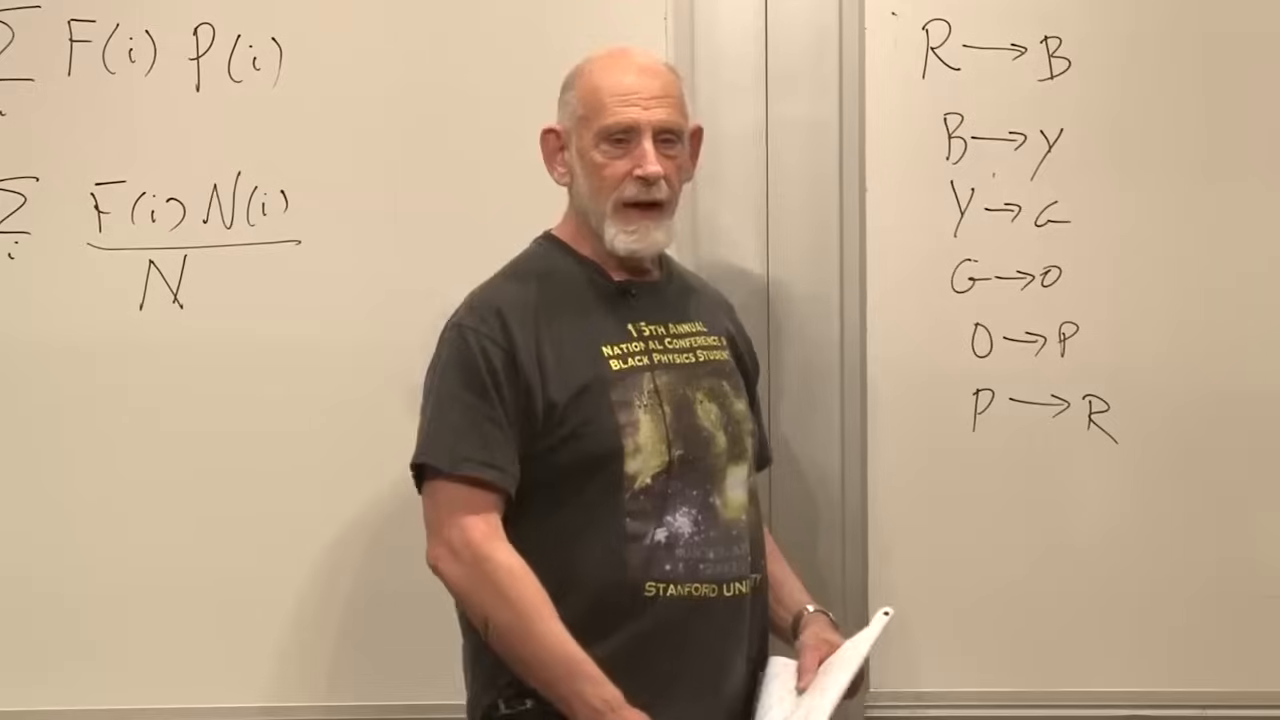
\includegraphics[width=0.92\textwidth]{lecture_01_figure_02.png}
\caption{Các công thức giá trị kỳ vọng vẫn ở bảng bên trái, còn sáu cập nhật màu tất định được liệt kê ở bên phải.}
\lectureframe{00:26:28}
\end{figure}

Danh sách trên bảng dễ hiểu hơn khi được vẽ thành một chu trình có hướng:
\begin{figure}[htbp]
\centering
\begin{tikzpicture}[
  >=Latex,
  state/.style={draw,circle,minimum size=8mm,inner sep=1pt}
]
\node[state] (R) at (90:2.2) {$R$};
\node[state] (B) at (30:2.2) {$B$};
\node[state] (Y) at (-30:2.2) {$Y$};
\node[state] (G) at (-90:2.2) {$G$};
\node[state] (O) at (-150:2.2) {$O$};
\node[state] (P) at (150:2.2) {$P$};
\draw[->] (R) -- (B);
\draw[->] (B) -- (Y);
\draw[->] (Y) -- (G);
\draw[->] (G) -- (O);
\draw[->] (O) -- (P);
\draw[->] (P) -- (R);
\end{tikzpicture}
\caption{Một quỹ đạo duy nhất gồm sáu trạng thái. Mỗi trạng thái được đi qua đúng một lần trong mỗi chu kỳ.}
\label{fig:sm1-six-cycle}
\end{figure}

Giả sử ta không biết trạng thái ban đầu và chụp một ảnh tức thời vào một thời điểm không biết. Vì mỗi bước kéo dài như nhau, hệ ở mỗi màu trong một phần sáu của chu kỳ:
\begin{equation}
 p(R)=p(B)=p(Y)=p(G)=p(O)=p(P)=\frac16.
 \label{eq:sm1-uniform-cycle}
\end{equation}
Sự bằng nhau này không đến từ hình dạng của vật. Nó đến từ việc thời gian hệ ở trong các trạng thái là như nhau.

Ta có thể sắp xếp lại các mũi tên và thu được một định luật vi mô khác mà vẫn tạo thành một chu trình gồm sáu trạng thái. Trình tự chi tiết thay đổi, nhưng xác suất của ảnh chụp tức thời vẫn là \(1/6\) vì mỗi trạng thái vẫn xuất hiện đúng một lần trong mỗi chu kỳ. Do đó, dự đoán này không cần biết điểm khởi đầu cũng không cần thứ tự chi tiết. Nó chỉ đòi hỏi cấu trúc quỹ đạo và thời gian bằng nhau cho mỗi lần cập nhật.

\begin{classroomqa}
\classquestion{Nếu vật không đối xứng, thì theo nghĩa nào việc gán cho mỗi màu xác suất \(1/6\) là hợp lệ?}
\lecturerresponse{Cách gán này mang tính động lực học chứ không phải hình học. Một ảnh chụp được lấy ở một pha chưa biết của một quỹ đạo sáu bước sẽ lấy mẫu sáu khoảng thời gian bằng nhau. Sự tương đương thích đáng ở đây là giữa các vị trí trên quỹ đạo, không phải giữa các mặt của vật. Nếu các thời gian lưu lại không bằng nhau, thì các xác suất cũng sẽ không bằng nhau.
\lecturetimestamp{00:27:11--00:29:49}}
\end{classroomqa}

\section{Các chu trình rời nhau và các đại lượng bảo toàn}

Một định luật tất định không nhất thiết đặt mọi trạng thái lên một quỹ đạo duy nhất. Hãy xét hai chu trình rời nhau,
\begin{equation}
 R\longrightarrow B\longrightarrow G\longrightarrow R,
 \qquad
 P\longrightarrow Y\longrightarrow O\longrightarrow P.
 \label{eq:sm1-two-cycles}
\end{equation}
Nếu ta biết rằng hệ nằm trên chu trình thứ nhất, thì
\begin{equation}
 \begin{aligned}
 p(R)=p(B)=p(G)&=\frac13,\\
 p(P)=p(Y)=p(O)&=0.
 \end{aligned}
\end{equation}
Biết rằng nó nằm trên chu trình thứ hai sẽ đảo ngược các cách gán này.

Trường hợp tổng quát hơn đòi hỏi các trọng số tiên nghiệm. Gán nhãn các chu trình là \(+1\) và \(-1\), và cho xác suất của chúng là \(p_+\) và \(p_-\), với
\begin{equation}
 p_++p_-=1.
\end{equation}
Khi đó,
\begin{align}
 p(R)=p(B)=p(G)&=\frac{p_+}{3},\\
 p(P)=p(Y)=p(O)&=\frac{p_-}{3}.
 \label{eq:sm1-sector-weights}
\end{align}
Các thừa số \(1/3\) suy ra từ chuyển động bên trong một chu trình. Các số \(p_+\) và \(p_-\) thì không. Chúng phải đến từ thông tin bổ sung, có lẽ từ một thí nghiệm khác hoặc một hệ khác chọn miền bảo toàn ban đầu.

Các nhãn \(+1\) và \(-1\) xác định một đại lượng bảo toàn: một khi hệ bắt đầu trên một chu trình, định luật cập nhật không bao giờ đưa nó sang chu trình kia. Ta có thể gọi đại lượng ấy là năng lượng, hoặc đặt cho nó một tên tạm như \emph{zilch}. Tên gọi của nó là thứ yếu. Bảo toàn có nghĩa là không gian trạng thái được chia thành các miền mà động lực học không thể vượt qua.

Các chu trình không nhất thiết phải chứa cùng một số trạng thái. Một quỹ đạo bốn trạng thái và một quỹ đạo hai trạng thái vẫn xác định hai miền bảo toàn. Khi đó, lấy mẫu theo các khoảng thời gian bằng nhau cho \(1/4\) trong miền thứ nhất và \(1/2\) trong miền thứ hai, trong mỗi trường hợp đều nhân với xác suất tiên nghiệm của miền đó. Cơ học thống kê phải trả lời hai câu hỏi tách biệt về mặt logic:
\begin{enumerate}
\item Trong một miền bảo toàn đã cho, động lực học dành bao nhiêu thời gian cho các trạng thái của nó?
\item Nên gán xác suất nào cho chính miền bảo toàn ấy?
\end{enumerate}

\begin{classroomqa}
\audiencequestion{Chúng ta có đang giả sử rằng mọi trạng thái bên trong một miền bảo toàn đều nhận cùng một xác suất không?}
\lecturerresponse{Đối với các định luật mô hình đơn giản rời rạc được trình bày ở đây, có, vì mỗi trạng thái tồn tại trong cùng một khoảng thời gian và chuyển động là tất định. Sự không biết nằm ở pha ban đầu của quỹ đạo. Một đầu dò có độ phân giải thời gian ở mức mili giây không thể phân biệt các lần cập nhật ở mức micro giây, mặc dù một ảnh chụp đủ nhanh vẫn có thể nhận diện trạng thái đã được chụp lại. Trong một hệ tổng quát hơn, các thời gian lưu lại không bằng nhau phải được tính đến một cách tường minh.
\lecturetimestamp{00:36:16--00:37:17}}
\end{classroomqa}

\begin{classroomqa}
\audiencequestion{Nếu lấy hai ảnh chụp tức thời và ảnh thứ nhất xác định một chu trình, thì ảnh thứ hai có nên xác định cùng chu trình đó không?}
\lecturerresponse{Có. Đó chính là ý nghĩa của bảo toàn. Một khi phép đo xác định giá trị của đại lượng bảo toàn, các xác suất trong tương lai có thể được điều kiện hóa theo giá trị đó, và các trạng thái trong miền kia nhận xác suất bằng không.
\lecturetimestamp{00:37:18--00:37:45}}
\end{classroomqa}

\subsection{Năng lượng được chia sẻ giữa hai hệ}

Bây giờ hãy thay nhãn trừu tượng bằng năng lượng. Một hộp cô lập là một hệ kín và có một năng lượng bảo toàn. Hai hộp cô lập có hai năng lượng được bảo toàn riêng rẽ vì chúng không tương tác. Nối chúng bằng một lối thông hẹp cho phép năng lượng chảy qua, và các năng lượng riêng rẽ có thể thay đổi trong khi tổng vẫn giữ cố định.

\begin{figure}[htbp]
\centering
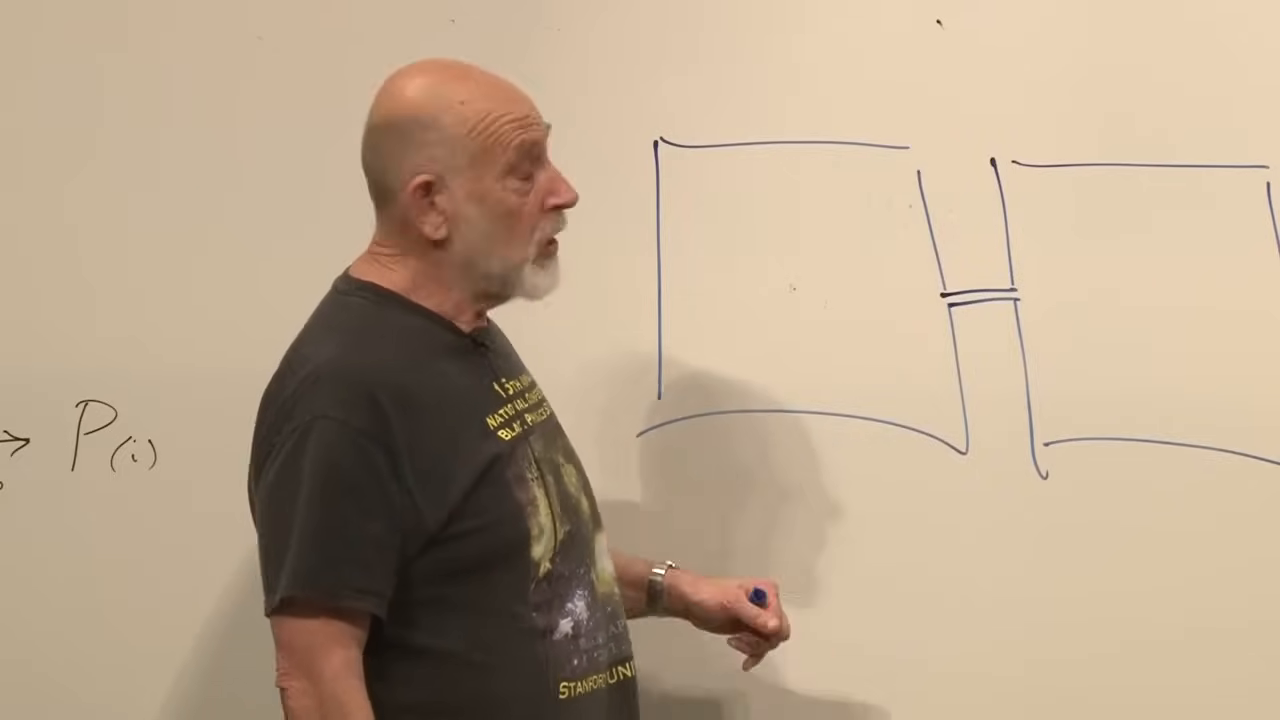
\includegraphics[width=0.92\textwidth]{lecture_01_figure_03.png}
\caption{Hai phân hệ được nối với nhau bằng một kênh hẹp mà qua đó năng lượng có thể truyền qua.}
\lectureframe{00:39:19}
\end{figure}

\begin{figure}[htbp]
\centering
\begin{tikzpicture}[>=Latex]
\draw[thick,rounded corners=4pt] (-4,1.8) rectangle (-0.7,-1.5);
\draw[thick,rounded corners=4pt] (0.7,1.5) rectangle (4,-1.8);
\draw[thick] (-0.7,0.45) -- (0.7,0.45);
\draw[thick] (-0.7,-0.35) -- (0.7,-0.35);
\draw[<->,very thick] (-0.45,0.05) -- (0.45,0.05);
\node at (-2.35,0.15) {subsystem \(1\)};
\node at (2.35,-0.15) {subsystem \(2\)};
\node[above] at (0,0.5) {energy exchange};
\end{tikzpicture}
\caption{Một khi mối nối được mở ra, chỉ còn \(E_1+E_2\) là được bảo toàn. Sự phân chia năng lượng trở thành một bài toán xác suất.}
\label{fig:sm1-connected-systems}
\end{figure}

Với một tổng năng lượng đã cho, ta có thể hỏi xác suất để phân hệ \(1\) có \(E_1\) trong khi phân hệ \(2\) có phần còn lại. Các hộp giống nhau trung bình phải có năng lượng bằng nhau, nhưng giá trị trung bình không phải là toàn bộ phân bố. Vì vậy, một cách để xác định các xác suất cho một phân hệ là đặt nó vào trong một hệ kín lớn hơn, mà định luật bảo toàn của hệ đó cung cấp thông tin còn thiếu. Cách xây dựng này sẽ còn lặp lại xuyên suốt cơ học thống kê.

\section{Các định luật tốt, các định luật xấu, và định luật âm thứ nhất}

Không phải mọi quy tắc cập nhật tất định đều có thể chấp nhận như một định luật cơ bản. Hãy xét ánh xạ
\begin{equation}
 \begin{aligned}
 R&\mapsto R,& B&\mapsto R,& Y&\mapsto R,\\
 G&\mapsto R,& O&\mapsto R,& P&\mapsto R.
 \end{aligned}
 \label{eq:sm1-all-to-red}
\end{equation}
Nó dự đoán tương lai một cách hoàn hảo: sau một bước, trạng thái là đỏ. Nó thất bại theo chiều ngược lại. Một khi hệ đã ở trạng thái đỏ, không có gì cho biết liệu nó đến từ xanh dương, vàng, xanh lục, cam, tím, hay từ chính đỏ.

\begin{figure}[htbp]
\centering
\begin{tikzpicture}[
  >=Latex,
  state/.style={draw,circle,minimum size=8mm,inner sep=1pt}
]
\node[state,fill=red!12] (R) at (0,0) {$R$};
\node[state] (B) at (-3,1.6) {$B$};
\node[state] (Y) at (-3,0) {$Y$};
\node[state] (G) at (-3,-1.6) {$G$};
\node[state] (O) at (3,1.6) {$O$};
\node[state] (P) at (3,-1.6) {$P$};
\draw[->] (B) -- (R);
\draw[->] (Y) -- (R);
\draw[->] (G) -- (R);
\draw[->] (O) -- (R);
\draw[->] (P) -- (R);
\draw[->,loop above] (R) to (R);
\end{tikzpicture}
\caption{Một định luật nhiều-đến-một dự đoán trạng thái kế tiếp nhưng xóa bỏ sự phân biệt giữa các trạng thái quá khứ khả dĩ.}
\label{fig:sm1-bad-law}
\end{figure}

Ngược lại, một chu trình kín bảo toàn dấu vết. Nếu biết thời gian đã trôi qua, ta có thể tiến hóa trạng thái theo chiều tiến hoặc chiều lùi, ngay cả sau nhiều nghìn chu kỳ. Định luật bảo toàn sự phân biệt giữa các điều kiện ban đầu. Susskind gọi yêu cầu này là \emph{định luật âm thứ nhất của vật lý}: thông tin không bị mất đi một cách căn bản.

Đối với một không gian trạng thái rời rạc hữu hạn, tiêu chuẩn bằng sơ đồ rất đơn giản:
\begin{quote}
Mỗi trạng thái của một định luật tốt có đúng một mũi tên đi ra và đúng một mũi tên đi vào.
\end{quote}
Mũi tên đi ra xác định tương lai; mũi tên đi vào tái dựng quá khứ. Về mặt toán học, phép cập nhật là một hoán vị của các trạng thái.

\subsection{Ma sát chỉ là một phản ví dụ biểu kiến}

Đối ứng liên tục là định lý Liouville. Ma sát dường như mâu thuẫn với nó. Hãy cho một cục tẩy trượt trên mặt bàn; dù nó bắt đầu ở đâu, cuối cùng nó cũng sẽ dừng lại. Một phương trình lực cản mang tính sơ đồ là
\begin{equation}
 m\ddot x=-\gamma\dot x,
 \qquad \gamma>0.
 \label{eq:sm1-drag}
\end{equation}
Vận tốc của nó suy giảm theo hàm mũ. Nếu đây là định luật nền tảng tối hậu của mọi hạt trong một căn phòng kín, thì mọi chuyển động đều sẽ tắt hẳn, nhiệt độ sẽ giảm về không, và nhiều trạng thái ban đầu sẽ sụp vào một trạng thái cuối cùng. Bảo toàn năng lượng sẽ không còn đúng, thông tin sẽ biến mất, và độ hỗn độn sẽ giảm đi. Đây sẽ là phiên bản liên tục của việc mọi thứ đều đi tới đỏ.

Ma sát thực không làm như vậy. Cục tẩy làm nóng mặt bàn, chính nó và môi trường xung quanh. Các vị trí và động lượng vi mô lưu lại những khác biệt đã mất khỏi chuyển động nhìn thấy được. Ma sát là một phương trình hiệu dụng cho một phân hệ sau khi đã lược bỏ các bậc tự do không quan sát được; nó không phải là một định luật tiêu tán cơ bản cho toàn bộ hệ kín.

\begin{classroomqa}
\classquestion{Phương trình vi phân \(m\ddot x=-\gamma\dot x\) biểu diễn điều gì, và vì sao nó không phải là một định luật cơ bản cho hệ kín?}
\lecturerresponse{Nó biểu diễn lực cản nhớt. Tự nó, nó kéo mọi vận tốc về không, điều đó sẽ làm cho một chất khí nguội xuống về không bất kể nhiệt độ ban đầu của nó. Trong một mô tả kín thực sự, năng lượng cơ học và thông tin bị mất sẽ chuyển vào các bậc tự do vi mô. Phương trình lực cản chỉ đáng tin cậy sau khi các biến đó đã được lược bỏ.
\lecturetimestamp{00:44:40--00:48:56}}
\end{classroomqa}

\section{Các trạng thái được chiếm và entropy đầu tiên}

Bảo toàn thông tin có một phát biểu xác suất tương đương. Giả sử \(M\) trong số \(N\) trạng thái được gán xác suất bằng nhau,
\begin{equation}
 p_i=
 \begin{cases}
 1/M, & i\text{ in the occupied set},\\
 0, & i\text{ outside it}.
 \end{cases}
 \label{eq:sm1-uniform-occupied}
\end{equation}
Một phép cập nhật bảo toàn thông tin có thể xáo lại những trạng thái nào được chiếm, nhưng nó không thể gộp chúng lại. Ở mọi thời điểm về sau vẫn còn \(M\) trạng thái, mỗi trạng thái có xác suất \(1/M\). Trái lại, ánh xạ xấu \eqref{eq:sm1-all-to-red} có thể làm nhiều trạng thái được chiếm sụp vào một trạng thái duy nhất.

Số \(M\) đo mức độ không biết của ta. Nếu \(M=N\), mọi trạng thái đều có thể và sự không biết của ta là cực đại. Nếu \(M=1\), trạng thái vi mô được biết chính xác. Vì thế định nghĩa đầu tiên của entropy là
\begin{equation}
 S=\log M.
 \label{eq:sm1-entropy-logm}
\end{equation}
Nó cho
\begin{equation}
 S_{\max}=\log N,
 \qquad
 S_{\min}=0.
\end{equation}
Nếu không gian trạng thái là vô hạn, thì có thể không tồn tại cận trên hữu hạn.

Trong cách phát triển này, entropy xuất hiện trước nhiệt độ, và thậm chí còn trước cả phát biểu hình thức của bảo toàn năng lượng. Theo nghĩa đó, nó cơ bản hơn. Tuy vậy, nó không phải chỉ là một tính chất của riêng hệ cơ học. Nó đồng thời phụ thuộc vào hệ và vào phân bố xác suất biểu diễn điều đã biết. Cùng một hệ cơ học có thể được những người quan sát có thông tin khác nhau gán các entropy khác nhau.

Dưới sự tiến hóa vi mô chính xác, các trạng thái được chiếm chỉ bị sắp xếp lại, nên entropy phân giải mịn này được bảo toàn. Trên thực tế, ta mất thông tin về thời điểm, bỏ qua các tương quan, và không thể theo dõi số lượng khổng lồ các biến. Khi đó phân bố xác suất của ta trải ra trên nhiều khả năng hơn, và entropy gán cho mô tả thô tăng lên. Các phương trình không nhất thiết phải hủy thông tin thì mô tả mà ta có thể sử dụng mới mất đi thông tin.

\begin{classroomqa}
\classquestion{Entropy lớn nhất có thể có của một hệ hữu hạn với \(N\) trạng thái là bao nhiêu?}
\lecturerresponse{Đó là \(\log N\), đạt được khi tất cả \(N\) trạng thái đều có xác suất như nhau. Entropy nhỏ nhất là 0, đạt được khi một trạng thái có xác suất bằng 1. Vì vậy entropy đo cả trạng thái hiểu biết lẫn không gian trạng thái khả dụng.
\lecturetimestamp{00:56:46--00:58:19}}
\end{classroomqa}

\section{Dòng Liouville trong không gian pha liên tục}

Đối với các hạt có vị trí và động lượng liên tục, một trạng thái vi mô là một điểm trong không gian pha. Ta ký hiệu các tọa độ là \(q_a\) và các động lượng liên hợp của chúng là \(p_a\). Với nhiều hạt thì có cực kỳ nhiều trục; một hình vẽ hai chiều với một \(q\) và một \(p\) chỉ là hình minh họa thay thế. Không gian pha có số chiều chẵn vì mỗi tọa độ đều có một động lượng đi kèm.

Giả sử tri thức của ta được biểu diễn bởi một miền \(\Omega_0\): mật độ xác suất đồng đều bên trong miền và bằng 0 ở bên ngoài. Chẳng hạn, biết rằng mọi hạt đều nằm trong phòng sẽ giới hạn các tọa độ vị trí, còn các cận về tốc độ của chúng sẽ giới hạn các tọa độ động lượng.

Sự tiến hóa Hamilton đưa mỗi điểm của không gian pha dọc theo một quỹ đạo. Các điểm lân cận chuyển tới các điểm lân cận, và vùng bị chiếm chảy như một khối chất lỏng không nén được:
\begin{figure}[htbp]
\centering
\begin{tikzpicture}[>=Latex,scale=0.95]
\draw[->] (-4.2,0) -- (4.3,0) node[right] {$q$};
\draw[->] (-3.7,-2.2) -- (-3.7,2.4) node[above] {$p$};
\draw[fill=blue!12,thick]
  (-3.0,-0.5) .. controls (-2.7,1.0) and (-1.3,1.2) .. (-0.9,0.1)
  .. controls (-0.6,-1.0) and (-2.2,-1.4) .. cycle;
\node at (-1.9,0.0) {$\Omega_0$};
\draw[->,very thick] (-0.3,0.2) -- (0.8,0.2);
\draw[fill=orange!15,thick]
  (1.2,-1.1) .. controls (1.5,0.3) and (2.3,1.8) .. (3.2,1.1)
  .. controls (3.6,0.7) and (2.8,-0.4) .. (2.5,-1.5)
  .. controls (2.1,-1.8) and (1.5,-1.6) .. cycle;
\node at (2.35,0.1) {$\Omega_t$};
\end{tikzpicture}
\caption{Dòng Hamilton có thể kéo giãn và cắt trượt một vùng không gian pha bị chiếm, nhưng vẫn bảo toàn thể tích của nó.}
\label{fig:sm1-liouville-flow}
\end{figure}

Định lý Liouville phát biểu rằng
\begin{equation}
 \operatorname{Vol}(\Omega_t)
 =
 \operatorname{Vol}(\Omega_0).
 \label{eq:sm1-liouville-volume}
\end{equation}
Nếu mật độ ban đầu đồng đều trên \(\Omega_0\), thì sau khi tiến hóa nó vẫn đồng đều trên \(\Omega_t\). Đây là tương tự liên tục của việc bảo toàn số lượng và trọng số của các trạng thái rời rạc được chiếm.

Định lý này cũng giải quyết bài toán ma sát theo cách hình học. Nếu chỉ nhìn vào động lượng nhìn thấy được của cục tẩy, một đám mây các khả năng dường như bị ép về phía \(p=0\). Trong không gian pha đầy đủ, đám mây ấy lan sang các vị trí và động lượng của các phân tử trong cục tẩy và mặt bàn. Một phép chiếu có thể co lại trong khi toàn bộ thể tích nhiều chiều vẫn không đổi.

\begin{classroomqa}
\classquestion{Nếu mọi quỹ đạo nhìn thấy được đều tiến tới trạng thái nghỉ, thì vùng không gian pha bị chiếm có sụp xuống trục \(p=0\) hay không?}
\lecturerresponse{Chỉ trong phép chiếu rút gọn. Hệ đầy đủ chứa các biến vi mô của mặt bàn, cục tẩy và môi trường xung quanh. Khi khoảng động lượng nhìn thấy được thu hẹp lại, phân bố lan ra theo những hướng ẩn đó. Định lý Liouville áp dụng cho toàn bộ không gian pha kín đầy đủ, chứ không áp dụng cho một tập biến vĩ mô không đầy đủ.
\lecturetimestamp{01:04:37--01:06:29}}
\end{classroomqa}

\section{Từ định luật âm một đến định luật thứ nhất}

\subsection{Một cái nhìn ngắn gọn về định luật thứ không}

Trước khi phát biểu định luật thứ nhất, sẽ hữu ích nếu nhắc đến định luật thứ không. Cân bằng nhiệt vẫn chưa được định nghĩa, nên lúc này định luật ấy chỉ là một phát biểu về cấu trúc:
\begin{quote}
Nếu hệ \(A\) cân bằng nhiệt với \(B\), và \(B\) cân bằng nhiệt với \(C\), thì \(A\) cân bằng nhiệt với \(C\).
\end{quote}
Tính bắc cầu này về sau sẽ cho phép định nghĩa nhiệt độ. Còn lúc này, ta tạm gác nó sang một bên.

\subsection{Bảo toàn năng lượng}

Định luật thứ nhất đối với một hệ kín đơn giản là
\begin{equation}
 \frac{dE}{dt}=0.
 \label{eq:sm1-first-law}
\end{equation}
Dạng súc tích của nó che khuất sức mạnh của nó. Năng lượng là một đại lượng bảo toàn, và từ năng lượng về sau sẽ mang nội dung nhiệt động lực học phong phú hơn.

Nếu một hệ kín gồm hai phần và năng lượng của chúng là cộng tính,
\begin{equation}
 E=E_1+E_2,
\end{equation}
thì
\begin{equation}
 \frac{dE_1}{dt}+\frac{dE_2}{dt}=0,
 \qquad\text{or}\qquad
 \frac{dE_1}{dt}=-\frac{dE_2}{dt}.
 \label{eq:sm1-energy-exchange}
\end{equation}
Dạng thứ hai làm cho sự trao đổi trở nên tường minh: năng lượng mà một hệ con mất đi chính là năng lượng mà hệ con kia nhận được.

Giả thiết cộng tính đòi hỏi phải cẩn thận. Hai hạt hấp dẫn nhau có các động năng riêng lẻ, nhưng tương tác của chúng đóng góp một thế năng thuộc về cả cặp. Tổng năng lượng vẫn được bảo toàn dù nó không thể được viết chính xác thành năng lượng của vật này cộng với năng lượng của vật kia.

Trong nhiệt động lực học, ta thường có thể dùng một xấp xỉ cộng tính rất tốt vì năng lượng khối tỉ lệ theo thể tích, trong khi năng lượng tương tác tầm ngắn giữa các phần lớn kề nhau chủ yếu tỉ lệ theo diện tích tiếp xúc của chúng. Hãy chia một cái bàn lớn thành các khối: nội năng của mỗi khối là một hiệu ứng thể tích, còn sự ghép giữa các khối kề nhau là một hiệu ứng bề mặt. Với các khối lớn, hiệu ứng sau nhỏ hơn một cách tương đối. Phương trình \eqref{eq:sm1-first-law} là chính xác cho toàn bộ hệ kín; dạng cho hệ con \eqref{eq:sm1-energy-exchange} giả sử năng lượng tương tác có thể bỏ qua.

\begin{classroomqa}
\audiencequestion{Điều kiện chuẩn hóa \(\sum_i p_i=1\) có đồng thời giả thiết rằng các kết quả được liệt kê loại trừ lẫn nhau hay không?}
\lecturerresponse{Có. Một nhãn trạng thái được định nghĩa sao cho các khả năng không chồng lấn lên nhau: nếu con xúc xắc ở trạng thái màu vàng, thì đồng thời nó không ở trạng thái màu đỏ. Trong ngôn ngữ thông thường các màu có thể được pha trộn, nhưng phân hoạch trạng thái dùng trong phép tính xác suất phải gồm các khả năng loại trừ lẫn nhau.
\lecturetimestamp{01:12:14--01:12:55}}
\end{classroomqa}

\section{Quay trở lại entropy}

Bài giảng giờ đây quay lại một cách tường minh với những điểm còn dang dở. Nhiệt độ, dù quen thuộc với giác quan, là một đại lượng dẫn xuất. Entropy và năng lượng phải được thiết lập trước thì mới có thể định nghĩa nhiệt độ một cách rành mạch.

\subsection{Các phân bố xác suất tổng quát}

Định nghĩa đặc biệt \(S=\log M\) áp dụng khi \(M\) trạng thái có xác suất bằng nhau và mọi trạng thái khác có xác suất bằng 0. Một phân bố tổng quát không nhất thiết phải có dạng hình chữ nhật. Các trọng số của nó có thể biến thiên trơn tru hoặc bất quy tắc theo các nhãn trạng thái.

\begin{figure}[htbp]
\centering
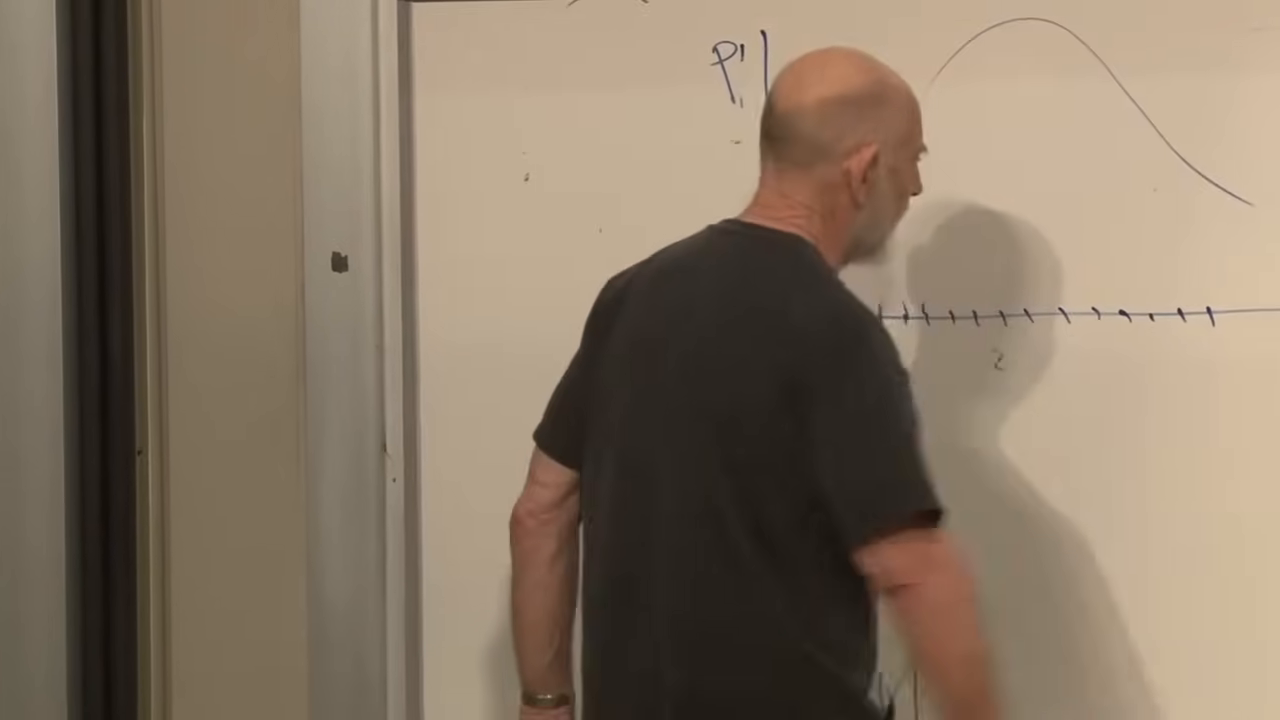
\includegraphics[width=0.92\textwidth]{lecture_01_figure_05.png}
\caption{Một phân bố xác suất được vẽ trên các nhãn trạng thái rời rạc. Điều cần cho entropy là độ trải rộng, chứ không phải chính xác hình dạng của đường cong.}
\lectureframe{01:14:40}
\end{figure}

\begin{figure}[htbp]
\centering
\resizebox{\linewidth}{!}{%
\begin{tikzpicture}[>=Latex,scale=0.93]
\draw[->] (-4.2,0) -- (4.4,0) node[right] {state label \(i\)};
\draw[->] (-4,0) -- (-4,3.2) node[above] {$p_i$};
\foreach \x in {-3.6,-3.1,...,3.6}
  \draw (\x,0.08) -- (\x,-0.08);
\draw[very thick]
  plot[smooth] coordinates {
  (-3.7,0.12) (-3.0,0.28) (-2.3,0.72) (-1.6,1.45)
  (-0.9,2.25) (-0.2,2.65) (0.5,2.28) (1.2,1.55)
  (1.9,0.88) (2.7,0.38) (3.5,0.14)};
\draw (-1.8,-0.18) -- (-1.8,-0.5);
\draw (1.8,-0.18) -- (1.8,-0.5);
\draw[<->] (-1.8,-0.46) -- (1.8,-0.46);
\node at (0,-0.82) {effective spread};
\end{tikzpicture}
}
\caption{Một phân bố hẹp mang ít bất định hơn một phân bố rộng. Entropy phải đo toàn bộ phân bố.}
\label{fig:sm1-probability-spread}
\end{figure}

Định nghĩa tổng quát là
\begin{equation}
 S=-\sum_i p_i\log p_i.
 \label{eq:sm1-shannon-entropy}
\end{equation}
Dùng \eqref{eq:sm1-expectation}, ta được
\begin{equation}
 S=-\langle\log p\rangle.
\end{equation}
Dấu trừ bù cho thực tế rằng \(\log p_i<0\) khi \(0<p_i<1\).

\subsection{Khôi phục kết quả của phân bố đồng đều}

Ta phải kiểm tra rằng công thức tổng quát tái tạo lại định nghĩa đầu tiên. Đối với một trạng thái không được chiếm, \(p_i=0\) còn \(\log p_i\) phân kỳ. Tích đó có giá trị giới hạn xác định rõ
\begin{equation}
 \lim_{p\to0^+}p\log p=0.
 \label{eq:sm1-plogp-limit}
\end{equation}
Vì thế các trạng thái có xác suất bằng 0 không đóng góp gì.

\begin{classroomqa}
\audiencequestion{Nếu \(p_i=0\), thì số hạng đó có thực sự bằng không không? Logarit của số không là âm vô cực.}
\lecturerresponse{Số hạng này được định nghĩa bởi giới hạn \(\lim_{p\to0^+}p\log p\), và giới hạn đó bằng không. Thừa số \(p\) tiến về không nhanh hơn logarit phân kỳ. Do đó, các trạng thái có xác suất nhỏ đến mức tùy ý cho những đóng góp nhỏ đến mức tùy ý, còn một trạng thái hoàn toàn không thể xảy ra thì không đóng góp gì.
\lecturetimestamp{01:18:27--01:19:46}}
\end{classroomqa}

Đối với mỗi trạng thái trong \(M\) trạng thái được chiếm, \(p_i=1/M\). Do đó
\begin{align}
 S
 &=-\sum_{\mathrm{occupied}\ i}
 \frac1M\log\!\left(\frac1M\right)\\
 &=-M\frac1M\log\!\left(\frac1M\right)\\
 &=-\log\!\left(\frac1M\right)
 =\log M.
 \label{eq:sm1-entropy-check}
\end{align}
Biểu thức tổng quát khớp chính xác với biểu thức đặc biệt. Một phân bố rộng hơn đặt trọng số đáng kể lên nhiều khả năng hơn nên có entropy lớn hơn; một phân bố hẹp hơn có entropy nhỏ hơn.

\begin{figure}[htbp]
\centering
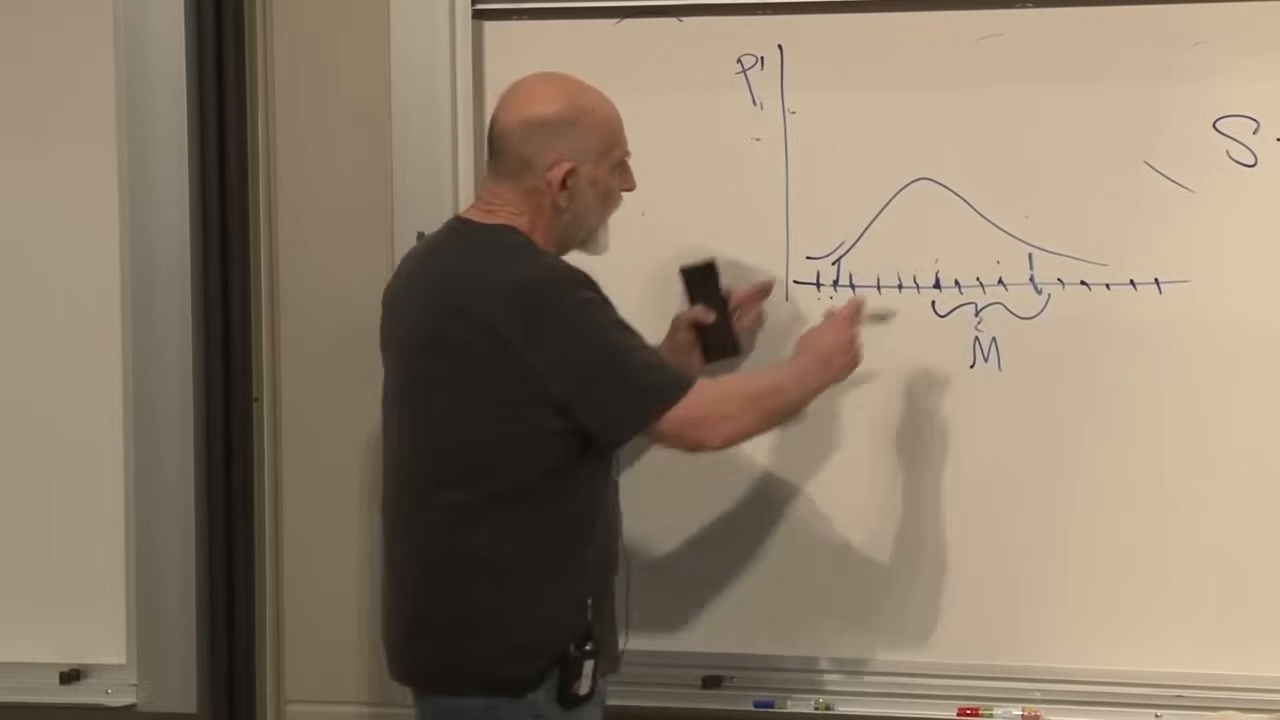
\includegraphics[width=0.92\textwidth]{lecture_01_figure_06.png}
\caption{Độ rộng được đánh dấu \(M\) nhấn mạnh mối liên hệ giữa độ trải của các xác suất đáng kể và entropy.}
\lectureframe{01:16:42}
\end{figure}

Entropy thuộc về một phân bố xác suất trên không gian trạng thái. Nó không phải là một đại lượng quan sát thuần túy như năng lượng hay động lượng của một vi trạng thái. Một trạng thái chính xác có thể được biểu diễn bằng một phân bố tập trung tại trạng thái đó và khi ấy có entropy bằng 0, nhưng entropy thay đổi khi trạng thái hiểu biết thay đổi.

\section{Đồng xu, bit và phép đếm tường minh}

Gọi \(n\) là số đồng xu. Số cấu hình vi mô là
\begin{equation}
 N=2^n.
 \label{eq:sm1-coin-state-count}
\end{equation}
Nếu không biết gì về các đồng xu, thì tất cả \(2^n\) cấu hình đều có xác suất như nhau, và
\begin{equation}
 S_{\max}=\log(2^n)=n\log2.
 \label{eq:sm1-coin-max-entropy}
\end{equation}
Entropy là cộng tính theo số đồng xu độc lập.

Với logarit cơ số \(2\), một hệ hai trạng thái hoàn toàn chưa biết có entropy bằng 1 bit. Với logarit tự nhiên, nó có entropy bằng \(\log2\). Đơn vị là quy ước; thứ tự và tính cộng tính cơ bản không đổi.

Ở cực kia, nếu mọi đồng xu đều đã biết, thì chính xác một cấu hình có xác suất bằng 1:
\begin{equation}
 S=0.
\end{equation}
Biết nhiều hơn nghĩa là entropy ít hơn.

Bây giờ giả sử chính xác một trong \(n\) đồng xu là sấp, còn tất cả các đồng xu khác đều ngửa, và vị trí của mặt sấp là chưa biết. Có \(n\) cấu hình có khả năng như nhau, mỗi cấu hình ứng với một vị trí khả dĩ của mặt sấp, nên
\begin{equation}
 S=\log n.
 \label{eq:sm1-one-tail-entropy}
\end{equation}
Nói chung đây không phải là bội số nguyên của \(\log2\). Bit là một đơn vị tiện lợi, chứ không phải khẳng định rằng mọi entropy đều xuất hiện theo các bậc nguyên bit.

\begin{classroomqa}
\audiencequestion{Có phải \(\log2\) chỉ xuất hiện vì mỗi đồng xu có hai trạng thái khả dĩ? Một phần tử có ba trạng thái thì sẽ cho \(\log3\) chứ?}
\lecturerresponse{Chính xác. Một phần tử hoàn toàn chưa biết với \(k\) trạng thái khả dĩ đóng góp \(\log k\). Các công tắc nhị phân đặc biệt thuận tiện trong máy tính vì các công tắc vật lý tự nhiên hiện thực hóa hai trạng thái ổn định và vì hai là số nguyên nhỏ nhất không tầm thường.
\lecturetimestamp{01:29:55--01:30:48}}
\end{classroomqa}

\begin{classroomqa}
\audiencequestion{Logarit ở đây được hiểu theo cơ số nào?}
\lecturerresponse{Trong các công thức vật lý này, \(\log\) có nghĩa là logarit tự nhiên. Các nhà lý thuyết thông tin thường dùng cơ số \(2\), nên entropy được đo trực tiếp bằng bit. Thay đổi cơ số chỉ nhân mọi entropy với cùng một hệ số chuyển đổi cố định và không làm thay đổi kết luận vật lý nào.
\lecturetimestamp{01:30:49--01:32:06}}
\end{classroomqa}

\section{Entropy trong không gian pha liên tục}

Quay lại không gian pha cổ điển \(\Gamma\). Nếu mật độ xác suất là đều trên một miền có thể tích \(V_\Gamma\) và bằng 0 ở bên ngoài, thì tương tự với việc đếm \(M\) trạng thái đồng khả năng là
\begin{equation}
 S=\log\!\left(\frac{V_\Gamma}{V_0}\right).
 \label{eq:sm1-continuous-uniform}
\end{equation}
Ở đây \(V_\Gamma\) là thể tích trong toàn bộ không gian nhiều chiều của các tọa độ và xung lượng, không phải thể tích không gian thông thường. Thể tích cố định \(V_0\) là một ô tham chiếu của không gian pha, làm cho logarit trở thành vô thứ nguyên. Đặt \(V_0=1\) thì cho cách viết tắt \(S=\log V_\Gamma\) được dùng trên bảng.

Đối với một mật độ xác suất tổng quát \(P(q,p)\), tổng rời rạc trở thành một tích phân trên không gian pha. Điều kiện chuẩn hóa là
\begin{equation}
 \int_\Gamma d\Gamma\,P(q,p)=1,
 \label{eq:sm1-continuous-normalization}
\end{equation}
và entropy là
\begin{equation}
 S=-\int_\Gamma d\Gamma\,
 P(q,p)\log\!\bigl[P(q,p)V_0\bigr].
 \label{eq:sm1-continuous-entropy}
\end{equation}
Mật độ là xác suất trên mỗi ô không gian pha. Về mặt khái niệm,
\eqref{eq:sm1-continuous-entropy} vẫn đo mức độ phân bố rộng của xác suất; đối với một vùng phân bố đều, nó thu về logarit của thể tích bị chiếm, đo theo đơn vị của ô tham chiếu. Thay đổi ô cố định đó làm tịnh tiến mọi entropy liên tục cùng một hằng số cộng và giữ nguyên các hiệu entropy.

\begin{classroomqa}
\audiencequestion{Vì sao ký hiệu tọa độ lại đổi từ \(x\) sang \(q\)?}
\lecturerresponse{Không có thay đổi vật lý nào. Cơ học cổ điển thường dùng hoặc \(x\) hoặc \(q\) cho các tọa độ và \(p\) cho các xung lượng liên hợp. Việc đổi ký hiệu chỉ là một sơ suất; cách xây dựng không gian pha là như nhau.
\lecturetimestamp{01:37:10--01:37:39}}
\end{classroomqa}

Nhiệt độ và phân bố Boltzmann được cố ý để lại sau. Nhiệm vụ tiếp theo sẽ là định nghĩa cân bằng nhiệt rồi xác định phân bố xác suất tương ứng.

\section{Các câu hỏi về tương quan, tính cộng và thông tin}

\subsection{Tương quan nghĩa là một phép đo làm thay đổi một phân bố khác}

Sự không biết gì hoàn toàn về các đồng xu độc lập gán xác suất bằng nhau cho mọi cấu hình. Khi đó, đo một đồng xu không cho ta biết gì về bất kỳ đồng xu nào khác. Các phân bố của chúng không thay đổi.

Ensemble có đúng một mặt sấp thì khác. Nếu đồng xu được đo ra mặt sấp, thì mọi đồng còn lại chắc chắn là mặt ngửa. Nếu đồng xu được đo ra mặt ngửa, thì mặt sấp duy nhất phải nằm trong \(n-1\) đồng còn lại, nên mỗi vị trí còn lại có xác suất có điều kiện
\begin{equation}
\begin{aligned}
 p(&\text{tail at a specified remaining position}\\
   &\mid\text{measured head})=\frac{1}{n-1}.
\end{aligned}
 \label{eq:sm1-conditional-tail}
\end{equation}
Đây là tương quan: biết một biến làm thay đổi phân bố xác suất được gán cho một biến khác.

\begin{classroomqa}
\audiencequestion{Trong các ví dụ về entropy có giả thiết các đồng xu độc lập với nhau không?}
\lecturerresponse{Chỉ khi sự không biết gì hoàn toàn được biểu diễn bằng các xác suất bằng nhau cho toàn bộ \(2^n\) cấu hình. Trong trường hợp đó, đo một đồng xu không làm thay đổi các phân bố của những đồng khác. Ví dụ một-mặt-sấp là trường hợp có tương quan tường minh: một phép đo cập nhật điều gì còn có thể xảy ra ở nơi khác. Thông tin đã nêu quyết định phân bố xác suất nào đang được dùng.
\lecturetimestamp{01:38:43--01:41:58}}
\end{classroomqa}

Ví dụ các chu trình rời nhau có cùng dạng lôgic. Việc đo nhãn được bảo toàn \(+1\) hoặc \(-1\) giới hạn mọi trạng thái về sau vào một phân khu. Điều kiện hóa theo thông tin được bảo toàn làm thay đổi phân bố được phép.

Entropy có tính cộng đối với các hệ không tương quan. Nếu
\begin{equation}
 p_{ij}=p_i^{(A)}p_j^{(B)},
\end{equation}
thì
\begin{align}
 S_{AB}
 &=-\sum_{i,j}p_i^{(A)}p_j^{(B)}
 \log\!\left[p_i^{(A)}p_j^{(B)}\right]\\
 &=S_A+S_B.
 \label{eq:sm1-entropy-additivity}
\end{align}
Các tương quan ngăn cản sự phân tích nhân tử này và làm giảm độ bất định độc lập của cả cặp.

Như một bài tập, hãy hình dung một hàng các biến nhị phân mà trong đó một trạng thái lên khiến mỗi láng giềng có xác suất ba phần tư ở trạng thái xuống. Đo một vị trí ngay lập tức làm thay đổi điều ta biết về các vị trí lân cận. Một phân bố như vậy là có tương quan, và entropy của nó không thể được tìm bằng cách cộng các entropy một-vị-trí cô lập mà không tính đến các tương quan đó.

\subsection{Boltzmann, Shannon và độ bất định lượng tử}

\begin{classroomqa}
\audiencequestion{Entropy nhiệt động học ra đời sớm hơn liên hệ thế nào với entropy lý thuyết thông tin của Shannon?}
\lecturerresponse{Cùng một dạng hàm xuất hiện trong cả hai:
\(-\sum_i p_i\log p_i\). Shannon thường dùng cơ số \(2\), còn các nhà vật lý thường dùng logarit tự nhiên và khôi phục hằng số Boltzmann khi entropy được biểu diễn theo đơn vị nhiệt động học. Khác biệt về mặt toán học chỉ là một hệ số chuyển đổi cố định, mặc dù các câu hỏi vật lý dùng để xác định các xác suất có thể rất khác nhau.
\lecturetimestamp{01:44:05--01:46:06}}
\end{classroomqa}

Đối với các vi trạng thái đồng khả năng, công thức nhiệt động học thường được viết
\begin{equation}
 S_{\mathrm{thermo}}=k_{\mathrm B}\log W,
 \label{eq:sm1-boltzmann-formula}
\end{equation}
trong đó \(W\) là số vi trạng thái khả dĩ có thể tiếp cận. Trong hệ đơn vị với \(k_{\mathrm B}=1\), đây chính xác là \(S=\log W\). Hằng số Boltzmann chuyển đổi giữa đơn vị nhiệt độ và đơn vị năng lượng; thang vi mô tự nhiên của nhiệt độ là năng lượng.

\begin{classroomqa}
\audiencequestion{Entropy này có đơn thuần chỉ là một dạng khác của nguyên lý bất định Heisenberg không?}
\lecturerresponse{Không. Entropy đang xét đo độ bất định trong một phân bố xác suất trên các trạng thái khả dĩ. Trong ngôn ngữ lượng tử, đó là độ bất định của một trạng thái hỗn hợp, không phải độ bất định nội tại của phép đo, vốn vẫn có thể còn tồn tại ngay cả đối với một trạng thái thuần. Cần giữ tách biệt hai khái niệm này.
\lecturetimestamp{01:46:07--01:47:31}}
\end{classroomqa}

\section{Những điều đã được thiết lập}

Điểm xuất phát không phải là tính ngẫu nhiên trong các định luật. Động lực học tất định, kết hợp với sự hiểu biết không đầy đủ về trạng thái ban đầu, đã tạo ra các xác suất. Một quỹ đạo đơn gán các trọng số thông qua thời gian lưu ở mỗi trạng thái; các quỹ đạo rời nhau bộc lộ các đại lượng bảo toàn và đòi hỏi các trọng số tiên nghiệm giữa các phân khu. Các định luật vi mô được chấp nhận bảo toàn các phân biệt; trong không gian trạng thái hữu hạn, điều đó có nghĩa là ở mỗi trạng thái có một mũi tên đi vào và một mũi tên đi ra, còn trong cơ học liên tục thì trở thành định lý Liouville.

Cấu trúc đó trước hết dẫn tới
\begin{equation}
 S=\log M
\end{equation}
cho \(M\) trạng thái được chiếm có xác suất bằng nhau, rồi tới
\begin{equation}
 S=-\sum_i p_i\log p_i,
\end{equation}
và cuối cùng tới tích phân trên không gian pha của nó. Entropy ghi nhận một phân bố xác suất và vì thế phản ánh một trạng thái hiểu biết. Thông tin hạt mịn được định luật vi mô bảo toàn ngay cả khi một mô tả thô hạt, mang tính thực dụng, không còn theo dõi được nó.

Bảo toàn năng lượng cho ta định luật thứ nhất, còn tính cộng của năng lượng các hệ con đòi hỏi năng lượng tương tác có thể bỏ qua. Entropy có tính cộng dưới một điều kiện tương ứng: các xác suất của các hệ con phải không tương quan. Hai kiểu tính cộng này chuẩn bị cho bước tiếp theo, nơi cân bằng nhiệt, nhiệt độ và phân bố Boltzmann sẽ nối năng lượng với xác suất.
